\begin{bibunit}[apalike]

\part[author={Stéphane GALLAND},label={chap:runtime_environments}]{Run-time Environments}

\tableofcontentslide

\section{Introduction}

\begin{frame}{Introduction}
	\begin{itemize}
	\item A compiler must implement the abstractions embodied in the source-language definition.
	\vfill
	\item \emph{The compiler must cooperate with the operating system and other systems software to support these abstracts on the target machine.}
	\vfill
	\item To do so, the compiler creates and manages a \Emph{run-time environment} in which it assumes its target programs are being executed.
	\vfill
	\item \alert{This chapter presents the key points of the run-time environment:}
		\begin{enumerate}
		\item Management of the Heap,
		\item Management of the Stack,
		\item Dynamic Memory Deallocation.
		\end{enumerate}
	\end{itemize}
\end{frame}

\section{Data Storage}

\tableofcontentslide[sectionstyle={show/shaded},subsectionstyle={show/show/hide},subsubsectionstyle={hide/hide/hide/hide}]

\begin{frame}{Storage Organization}
	\begin{itemize}
	\item The target program runs in its own \emph{logical address space} in which each value has a location.
	\item The organization and management of this logical address space is shared between: \begin{itemize}
		\item the compiler,
		\item the operating system,
		\item the target machine.
		\end{itemize}
	\vfill
	\item The operating system maps the logical addresses into physical addresses.
	\item When defined, a \emph{virtual machine} is a program that is representing the operating system and the target machine into an abstract and platform-independent machine.
	\end{itemize}
\end{frame}

\sidecite{Randell.1964}
\begin{frame}[t]{Structure of the Logicial Address Space}
	\begin{itemize}
	\item In the run-time environment, the logical address space has a structure; typically:
	\end{itemize}
	\vfill
	\begin{columns}
		\begin{column}{.3\linewidth}
			\raisebox{-.5\height}{\includeanimatedfigure[width=\linewidth]{address_space_structure}}
		\end{column}
		\begin{column}{.7\linewidth}\begin{small}
			\only<2>{\begin{itemize}
				\item The compiler can place the executable target code in a statically determined area, named Code.
				\item This area contains the binary representations of the instructions to execute.
				\item The format of the code depends on the target machine: Intel binary assembler, byte code\dots
				\end{itemize}}
			\only<3>{\begin{itemize}
				\item Similarly, the size of some program data may be known at compile time.
				\item The area where these data are stored in named Static area, usually put just after the Code area.
				\item \inlineexamples{string literals, global constants and variables, information related to garbage collection\dots}
				\item The addresses of the static data are directly put in the code.
				\end{itemize}}
			\only<4>{\begin{itemize}
				\item The stack is used to store data structures called activation records.
				\item Activation records are generated during the procedure/function calls (explained later).
				\item Basically, each record contains the status of the machine: ordinal counter, machine registers, and data whose lifetimes are the same as the activation time (usually local variables).
				\end{itemize}}
			\only<5>{\begin{itemize}
				\item Many languages allow the programmer to allocate and deallocate data under program control (malloc, new\dots)
				\item The heap is used to manage this kind of long-lived data.
				\end{itemize}}
			\only<6>{\begin{itemize}
				\item The heap and the stack are growing up and consume the free memory space between them.
				\item When the stack cannot grow up, the classical ``stack overflow'' error is fired.
				\item When the heap cannot grow up, the classical ``out of memory'' error is fired.
				\end{itemize}}
			\end{small}
		\end{column}
	\end{columns}
\end{frame}

\begin{frame}{Static vs. Dynamic Storage Allocation}
	The layout and allocation of data to memory locations in the run-time environment are key issues in storage management.
	\vfill
	\begin{block}{Static Storage Allocation}
		It is made \emph{by the compiler} looking only at the text of the program, not at what the program does when it executes.
	\end{block}
	\vfill
	\begin{block}{Dynamic Storage Allocation}
		\begin{itemize}
		\item It is made only \emph{while the program is running}.
		\item Many compilers use a combination of the strategies explained in the following slide for dynamic storage allocation.
		\end{itemize}
	\end{block}
\end{frame}

\sidecite{Randell.1964}
\begin{frame}{Strategies for Dynamic Storage Allocation}
	\begin{block}{Stack Storage}
		\begin{itemize}
		\item Names local to a procedure are allocated space \emph{on a stack}.
		\item The stack supports the normal call/return policy for procedures.
		\end{itemize}
	\end{block}
	\vfill
	\begin{block}{Heap Storage}
		\begin{description}
		\item Data that may outlive the call to the procedure that created it is usually allocated \emph{on a ``heap''} of reusable storage.
		\item The heap is an area of virtual memory that allows data to obtain and release storage.
		\item[Garbage collection] the run-time environment detects useless data in heap and releases them.
		\end{description}
	\end{block}
\end{frame}

\section{Stack management}

\tableofcontentslide[sectionstyle={show/shaded},subsectionstyle={show/show/hide},subsubsectionstyle={hide/hide/hide/hide}]

\subsection{Stack allocation}

\subsubsection{Introduction}

\tableofcontentslide[sections={1-4},sectionstyle={show/shaded},subsectionstyle={show/shaded/hide},subsubsectionstyle={show/show/hide/hide}]

\sidecite{Randell.1964}
\begin{frame}{Stack Allocation}
	\begin{description}
	\item Compilers that use procedures, functions, or methods as units manage a part of their run-time memory as a stack.
	\item[Note] procedure will be used as a generic term for procedure, function and method.
	\vfill
	\item Each time a procedure is called:
		\begin{itemize}
		\item space for its local variables is pushed into a stack.
		\end{itemize}
	\item When the procedure terminates:
		\begin{itemize}
		\item space is popped off the stack.
		\end{itemize}
	\vfill
	\item The activation of procedure $\equiv$ the call to the procedure.
	\end{description}
\end{frame}

\begin{frame}[fragile]{Nested Activation in Time}
	\begin{small}
	\alertbox{Stack allocation would not be feasible if procedure calls did not nest in time.}
	\begin{columns}
		\begin{column}{.5\linewidth}
			\begin{itemize}
			\item If an activation of procedure \code{p} calls procedure \code{q}, then that activation of \code{q} must end before the activation of \code{p} can end.
			\end{itemize}
			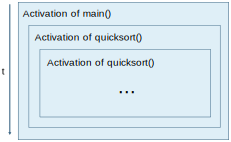
\includegraphics[width=\linewidth]{nested_activation}
		\end{column}
		\begin{column}{.5\linewidth}
			\begin{lstlisting}[language=C,basicstyle=\Tiny]
			int a[11];
			void readArray() {
			    int i; // read and fill a
			}
			int partition(int m, int n) {
			    // let v, a[m..p-1] < v, a[p]=v, a[p+1..n] >= v
			    // return p
			}
			void quicksort(int m, int n) {
			    int i;
			    if (n>m) {
			        i = partition(m,n);
			        quicksort(m,i-1);
			        quicksort(i+1,n);
			    }
			}
			main() {
			    readArray();
			    a[0] = -9999;
			    a[11] = 9999;
			    quicksort(1,9);
			}
			\end{lstlisting}
		\end{column}
	\end{columns}
	\end{small}
\end{frame}

\begin{frame}[allowframebreaks]{Termination of Nested Activation}
	Three common cases when \code{p} calls \code{q}:
	\vspace{1em}
	\begin{enumerate}
	\item[Normal] The activation of \code{q} terminates normally. Then in essentially any language, control resumes just after the point of \code{p} at which the call to \code{q} was made.
	\vspace{1em}
	\item[Abort] The activation of \code{q}, or some procedure called by \code{q}, either directly or indirectly, aborts.
\code{p} ends simultaneously with \code{q}.
	\item[Exception] The activation of \code{q} terminates because of an exception that \code{q} cannot handle. \\
		Procedure \code{p} may handle the exception: the activation of \code{q} has terminated but \code{p} continues (not necessary where \code{q} was called). \\
		If \code{p} cannot handle the exception, then this activation of \code{p} terminates at the same time as the activation of \code{q}, and presumably, the exception will be handled by some other open activation of a procedure.
	\end{enumerate}
\end{frame}

\subsubsection{Activation tree}

\tableofcontentslide[sections={1-4},sectionstyle={show/shaded},subsectionstyle={show/shaded/hide},subsubsectionstyle={show/shaded/hide/hide}]

\begin{frame}{Activation Tree}
	The activations of procedures during the running of an entire program is represented by a tree, named \emph{activation tree}.
	\vfill
	\begin{description}
	\item[Node] an activation;
	\vfill
	\item[Root Node] the root is the activation of the ``main'' procedure that initiates the execution of the program.
	\vfill
	\item[Child Node] activations of the procedures called by the activation represented by the parent node. The order of the children (from left to right) is the order of the activations.
	\end{description}
\end{frame}

\figureslide{Example of Activation Tree}{activation_tree_example}

\subsubsection{Control Stack and Activation record}

\tableofcontentslide[sections={1-4},sectionstyle={show/shaded},subsectionstyle={show/shaded/hide},subsubsectionstyle={show/shaded/hide/hide}]

\begin{frame}{Control Stack and Activation Record}
	\begin{itemize}
	\item Procedure calls and returns are usually managed by a run-time stack called the \emph{control stack}.
	\vfill
	\item Each live activation has an \emph{activation record} (or frame) on the control stack.
	\vfill
	\item The entire sequence of activation records on the stack corresponding to the path in the activation tree to the activation where control currently resides.
	\vfill
	\item \emph{The latter activation has its record at the top of the stack.}
	\end{itemize}
\end{frame}

\figureslide{Example of Control Stack}{control_stack_example}

\begin{frame}[t]{Structure of the Activation Record}
	\begin{itemize}
	\item The contents of activation records vary with the language being implemented; typically:
	\end{itemize}
	\vfill
	\begin{columns}
		\begin{column}{.3\linewidth}
			\raisebox{-.5\height}{\includeanimatedfigure[width=\linewidth]{activation_record_structure}}
		\end{column}
		\begin{column}{.7\linewidth}\begin{small}
			\only<2>{\begin{itemize}
				\item Temporary values, such as those arising from the evaluation of expressions, in cases where the temporaries cannot be held in registers.
				\end{itemize}}
			\only<3>{\begin{itemize}
				\item Local data belonging to the procedure whose activation record this is.
				\end{itemize}}
			\only<4>{\begin{itemize}
				\item Information about the state of the machine just before the call to the procedure.
				\item It typically includes:
					\begin{description}
					\item[return address] the value of the ordinal counter to which the called procedure must return.
					\item[Registers] The contents of registers that were used by the calling procedure and that must be restored when the return occurs.
					\end{description}
				\end{itemize}}
			\only<5>{\begin{itemize}
				\item An ``access link'' may be needed to locate data needed by the called procedure but found elsewhere (in another activation record\dots)
				\end{itemize}}
			\only<6>{\begin{itemize}
				\item A ``control link'' is pointing to the activation record of the caller.
				\end{itemize}}
			\only<7>{\begin{itemize}
				\item Space for the return value of the called function, if any.
				\item Not all called procedures return a value.
				\item We may prefer to place that value in a register for efficiency.
				\end{itemize}}
			\only<8>{\begin{itemize}
				\item The actual parameters are given by the caller and used by the callee procedure.
				\item Commonly, these values are not placed in the activation record but rather in registers, when possible.
				\end{itemize}}
			\end{small}
		\end{column}
	\end{columns}
\end{frame}

\subsubsection{Calling sequence}

\tableofcontentslide[sections={1-4},sectionstyle={show/shaded},subsectionstyle={show/shaded/hide},subsubsectionstyle={show/shaded/hide/hide}]

\sidecite{Johnson.1981}
\begin{frame}{Calling and Return Sequence}
	\begin{definition}[Calling Sequence]
		A calling sequence is a \code{code} that allocates an activation record on the stack and enters information into its fields.
	\end{definition}
	\begin{definition}[Return Sequence]
		A return sequence is a \code{code} that deallocates an activation record from the stack and restores the state of the machine.
	\end{definition}
	\vfill
	\alertbox{Calling sequences and the layout of activation records may differ greatly, even among implementations of the same language.}
	\vfill
	\begin{itemize}
	\item The calling sequence is composed of: \begin{itemize}
		\item Calling procedure (the ``caller''),
		\item Called procedure (the ``callee'').
		\end{itemize}
	\end{itemize}
\end{frame}

\sidecite{Randell.1964}
\begin{frame}[t]{Principles of the Calling Sequences}
	\putat(180,-200){\includeanimatedfigure[width=.4\paperwidth]{calling_sequence_principles}}
	When designing calling sequences and the layout of the activation records, the following principles are used:
	\only<1>{\begin{enumerate}
		\item \emph{Values communicated between caller and callee are generally placed at the beginning of the callee activation record.}
		\end{enumerate}}
	\only<2>{\begin{enumerate}
		\setcounter{enumi}{1}
		\item \emph{Fixed-length items are placed in the middle of the record.}
		\end{enumerate}}
	\only<3>{\begin{enumerate}
		\setcounter{enumi}{2}
		\item \emph{Items whose size may not be known early enough are placed at the end of the activation record.}
		\end{enumerate}}
	\only<4>{\begin{enumerate}
		\setcounter{enumi}{3}
		\item \emph{We must locate the ``top-of-stack'' pointer judiciously.}
		\end{enumerate}}
	\vspace{1em}
	\hspace{2em}\begin{minipage}{.5\linewidth}
		\only<1>{	\small
				\nohyphens{The caller can compute the actual parameters and put them at the top of the stack, without the necessity to create the entire record of the callee, and knowing how the callee's record layout is.}
				\par
				\nohyphens{The caller knows where to put the return value, relative to its own record.}
		}
		\only<2>{	\small
				\nohyphens{If machine status are standardized, then programs such as debuggers will have an easier time deciphering the stack contents if an error occurs.}
		}
		\only<3>{	\small
				\nohyphens{Most of the variables have a size that can be determined by the compiler. But some cannot (dynamic arrays\dots)}
				\par
				\nohyphens{The amount of space needed for temporaries is not known during the first phase of the intermediate code generation.}
		}
		\only<4>{	\small
				\nohyphens{Commonly, it points to the end of the fixed-length fields in the activation record.}
				\par
				\nohyphens{The control link points to the ``top-of-stack'' of the previous record.}
				\par
				\nohyphens{Fixed-length data can then be accessed by fixed negative offset, and variable-length with a run-time positive offset.}
		}
	\end{minipage}
\end{frame}

\begin{frame}{Typical Calling Sequence}
	\begin{enumerate}
	\item The caller evaluates and stores the actual parameters
	\item The caller stores a return address. \\
		It stores the old value of the \code{top\_sp} into the callee's activation record. \\
		It increments \code{top\_sp} to point to the callee activation record.
	\item The callee saves the register values and other status information.
	\item The callee initializes its local data and begins execution.
	\end{enumerate}
	\putat(-20,-175){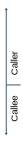
\includegraphics[width=2em]{caller_callee}}
\end{frame}

\begin{frame}{Typical Return Sequence}
	\begin{enumerate}
	\item The callee places the return value next to the parameters.
	\item Using information in the machine-status fields, the callee restores \code{top\_sp} and other registers. \\
		It branches to the return address that the caller placed in the status field.
	\item Although \code{top\_sp} has been decremented, the caller knows where the return value is, relative to the current value of \code{top\_sp}. \\
		The caller may use that value.
	\end{enumerate}
	\putat(-20,-172){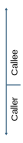
\includegraphics[width=2em]{callee_caller}}
\end{frame}

\subsubsection{Variable-length data on the stack}

\tableofcontentslide[sections={1-4},sectionstyle={show/shaded},subsectionstyle={show/shaded/hide},subsubsectionstyle={show/shaded/hide/hide}]

\begin{frame}{Variable-length Data}
	\begin{itemize}
	\item Programs contain a lot of data whose \Emph{sizes are known at run-time}; but which are local to a procedure.
	\item Because \Emph{they are local to the procedure}, they may be allocated on the stack.
	\vfill
	\item In most of the modern languages, these objects are allocated in the \emph{heap}.
	\item However, it is also possible to allocate objects, arrays, or other data structures of unknown size on the \emph{stack}.
	\end{itemize}
	\vfill
	\begin{block}{Why on the stack?}
		Avoiding the expense of garbage collecting the space allocated for the variable-length data.
	\end{block}
\end{frame}

\pgfdeclareimage[width=.3\paperwidth]{stack_allocation_strategy}{imgs/chapter5/stack_allocation_strategy}

\begin{frame}[fragile]{Allocation Strategy}
	\putat(180,-140){\pgfuseimage{stack_allocation_strategy}}
	\begin{itemize}
	\item Below, the example of programs in C99 and C\# in which a local array is declared. Its size depends on the value of the procedure parameter.
	\end{itemize}
	\begin{minipage}{.5\linewidth}
	\begin{itemize}
	\item The common strategy is to:
		\begin{enumerate}
		\item Allocate the arrays at the end of the record.
		\item Put pointers to the allocated regions in the local data.
		\end{enumerate}
	\end{itemize}
	\end{minipage} \\
	\vspace{2em}
	\begin{columns}
		\begin{column}{.5\linewidth}
			\begin{lstlisting}[language=c]
			/* C99 */
			void myFunction(int n) {
			   float localArray[n];
			   /* Do something with array */
			}
			\end{lstlisting}
		\end{column}
		\begin{column}{.5\linewidth}
			\begin{lstlisting}[language=c]
			/* C# */
			unsafe void myFunction(int n) {
			   int* localArray = stackalloc int[size];
			   /* Do something with array */
			}
			\end{lstlisting}
		\end{column}
	\end{columns}
\end{frame}

\begin{frame}{Pointers \code{top} and \code{top\_sp}}
	\begin{itemize}
	\item Two pointers are used:
		\begin{description}
		\item[top] marks the actual top of the stack. It points to the position at which the next activation record will begin.
		\item[top\_sp] is used to find local, fixed-length fields of the top activation record.
		\end{description}
	\vfill
	\item When returning from a call: \\
		\code{top $\leftarrow$ top\_sp - length(fixed\_record\_part)}
	\end{itemize}
	\vfill
	\begin{center}
		\pgfuseimage{stack_allocation_strategy}
	\end{center}
\end{frame}

\subsection{Access to nonlocal data on the stack}

\subsubsection{Introduction}

\tableofcontentslide[sections={1-4},sectionstyle={show/shaded},subsectionstyle={show/shaded/hide},subsubsectionstyle={show/show/hide/hide}]

\begin{frame}{Access to Nonlocal Data on the Stack}
	\begin{itemize}
	\item This section is devoted to the mechanisms of the procedures to access to their data.
	\item Focusing on the mechanisms for finding data used within a procedure p but that does not belong to p.
	\vfill
	\item First, we study the cases of programs without nested functions.
	\item Second, we introduces an algorithmic languages that permits to declare nested functions.
	\end{itemize}
\end{frame}

\subsubsection{Data access without nested procedure}

\tableofcontentslide[sections={1-4},sectionstyle={show/shaded},subsectionstyle={show/shaded/hide},subsubsectionstyle={show/shaded/hide/hide}]

\begin{frame}{Data Access Without Nested Procedures}
	\begin{itemize}
	\item In languages similar to C, variables are declared:
		\begin{itemize}
		\item inside a single function, or
		\item outside any function (``globally'')
		\end{itemize}
	\vfill
	\item It is impossible to declare a procedure inside the scope of another procedures.
	\vfill
	\item In such languages, allocation of storage for, and access to variables is simple:
		\begin{itemize}
		\item \emph{Global variables are allocated in the static storage.} The locations remain fixed and are known at compile time.
		\item \emph{Any other name must be local to the activation at the top of the stack.} The locations are relative to the \code{top\_sp} pointer of the stack.
		\end{itemize}
	\end{itemize}
\end{frame}

\subsubsection{Issues with nested procedures}

\tableofcontentslide[sections={1-4},sectionstyle={show/shaded},subsectionstyle={show/shaded/hide},subsubsectionstyle={show/shaded/hide/hide}]

\begin{frame}[fragile]{Language with Nested Procedure Declarations}
	\begin{itemize}
	\item Many languages enable to declare procedures inside the scope of another procedure (Algol60, Pascal, ML, LISP).
	\item LISP is a functional language: variables, after initialized cannot change.
	\end{itemize}
	\vfill
	\begin{columns}
		\begin{column}{.4\linewidth}
			Factorial Function, non-tail-recursion algorithm. \\
			\vspace{3em}
			Factorial Function, tail-recursion algorithm.
		\end{column}
		\begin{column}{.6\linewidth}
			\begin{lstlisting}[language=lisp,basicstyle=\footnotesize]
			(deffun factorial (n)
				(if (<= n 1)
				    1
				    (* n factorial (- n 1))))

			(deffun factorial (n)
				(let ((deffun fact (n,acc)
					      (if (<= n 1) acc
					          (fact (- n 1) (* n acc))))
				     (fact n 1)))
			\end{lstlisting}
		\end{column}
	\end{columns}
\end{frame}

\begin{frame}{Issue with Nested Procedures}
	\begin{footnotesize}
	\alertbox{With nested procedure declaration, it is far more complicated to determine the addresses of the names used in the procedure.}
	\vfill
	\begin{example}
		\begin{columns}
			\begin{column}[t]{.6\linewidth}
				\begin{itemize}
				\item Let the procedure \code{g} declared inside the scope of the procedure \code{p}.
				\item \code{g} is accessing to the variable \code{a}, locally declared in \code{p}.
				\item It is difficult to determine at compile time where is the variable \code{a} in the stack, because of the recursive calls.
				\item The address of \code{a} in the stack can be determined only at run-time.
				\end{itemize}
			\end{column}
			\begin{column}[t]{.4\linewidth}
				\begin{scriptsize}
				\begin{myprocedure}{p}{n}
				\Begin{
					\KwSty{Declare} a \affect n/2\;
					\KwSty{Procedure} {g()} \\
					\Begin{
						\lIf{$n>1$}{p(n-1)\;}
						\lElseIf{$n=1$}{p(a/2)\;}
					}
					g() \;
				}
				\end{myprocedure}
				\end{scriptsize}
			\end{column}
		\end{columns}
	\end{example}
	\end{footnotesize}
\end{frame}

\figureslide{Example of the Issue}{nested_procedure_issue}

\subsubsection{Nesting depth}

\tableofcontentslide[sections={1-4},sectionstyle={show/shaded},subsectionstyle={show/shaded/hide},subsubsectionstyle={show/shaded/hide/hide}]

\begin{frame}{Informal Definition of Nesting Depth}
	\begin{itemize}
	\item Let nesting depth $1$ the declaration of a procedure outside another procedure.
	\item Let nesting depth $2$ the declaration of a procedure inside one other procedure of nesting depth $1$.
	\item Let nesting depth $n$ the declaration of a procedure inside one other procedure of nesting depth $n-1$.
	\end{itemize}
	\begin{columns}
		\begin{column}{.3\linewidth}
			\begin{scriptsize}
			\begin{myprocedure}{p}{n}
			\Begin{
				\KwSty{Declare} a \affect n/2\;
				\KwSty{Procedure} {g()} \\
				\Begin{
					\lIf{$n>1$}{p(n-1)\;}
					\lElseIf{$n=1$}{p(a/2)\;}
				}
				g() \;
			}
			\end{myprocedure}
			\end{scriptsize}
		\end{column}
		\begin{column}{.35\linewidth}
			\begin{small}
			\code{p} has nesting depth $1$. \\
			\vspace{2em}
			\code{g} has nesting depth $2$.
			\end{small}
		\end{column}
	\end{columns}
\end{frame}

\subsubsection{Access links}

\tableofcontentslide[sections={1-4},sectionstyle={show/shaded},subsectionstyle={show/shaded/hide},subsubsectionstyle={show/shaded/hide/hide}]

\begin{frame}{Access Link}
	\begin{small}
	\begin{definition}
		Access links provide a mean for the implementation of the static scope rule for nested functions.
	\end{definition}
	\begin{description}
	\item If procedure \code{g} is immediately nested in procedure \code{p}; then the access link in any activation of \code{g} points to the most recent activation of \code{p}.
	\item[Note] nesting depth of \code{p} must be exactly one less than the nesting depth of \code{g}.
	\end{description}
	\end{small}
	\begin{columns}
		\begin{column}{.5\linewidth}
			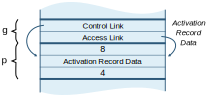
\includegraphics[width=\linewidth]{access_link}
		\end{column}
		\begin{column}{.3\linewidth}
			\begin{tiny}
			\begin{myprocedure}{p}{n}
			\Begin{
				\KwSty{Declare} a \affect n/2\;
				\KwSty{Procedure} {g()} \\
				\Begin{
					\lIf{$n>1$}{p(n-1)\;}
					\lElseIf{$n=1$}{p(a/2)\;}
				}
				g() \;
			}
			\end{myprocedure}
			\end{tiny}
		\end{column}
	\end{columns}
\end{frame}

\begin{frame}{Chain of Access Links}
	\begin{itemize}
	\item Access links form a chain from the activation record at the top of the stack to a sequence of activations at progressively lower nesting depths.
	\vfill
	\item Along this chain are all the activations whose data and procedures are accessible to the currently executing procedure.
	\end{itemize}
\end{frame}

\begin{frame}{Example of Access Links}
	\putat(160,-75){\parbox{.5\linewidth}{\normalcolor\mdseries
		\begin{tiny}
		\begin{myprocedure}{sqrt}{q}
		\Begin{
			\KwSty{Procedure} {babylonian\_algo(a,n)} \\
			\Begin{
				\KwSty{Declare} {a}\;
				b \affect (a + q/a) / 2\;
				\uIf{n {\textgreater} 0}{
					\Return {b}\;
				}
				\Else{
					\Return {babylonian\_algo(a,n-1)}\;
				}
			}
			\Return{babylonian\_algo(q/2, 10)}\;
		}
		sqrt(5)\;
		\end{myprocedure}
		\end{tiny}
	}}
	\putat(160,-170){\only<4>{\parbox{.5\linewidth}{\normalcolor\mdseries
		\small\nohyphens{To access to the value of \code{q}, we know at compile time, that it is reachable after one dereferencing in the access link pointer chain.}
	}}}
	\putat(-20,-190){\includeanimatedfigure[width=.5\paperwidth]{access_link_example}}
\end{frame}

\begin{frame}[t]{Determining the Access Link Target}
	\begin{small}
	\begin{itemize}
	\item Let the procedure \code{q} calling \code{p}.
	\item Let $N_\alpha$ the nesting depth of $\alpha$.
	\item Let $D_\beta$ the set of the nesting procedures in which $\beta$ is defined.
	\end{itemize}
	\end{small}
	\begin{block}{First Case}
		\[ \left( N_p > N_q \right) \Rightarrow \left( q \in D_p \wedge N_p = N_q + 1 \right) \]
		Then the access link from \code{p} leads to \code{q}.
	\end{block}
\end{frame}

\begin{frame}[t]{Determining the Access Link Target}
	\begin{small}
	\begin{itemize}
	\item Let the procedure \code{q} calling \code{p}.
	\item Let $N_\alpha$ the nesting depth of $\alpha$.
	\item Let $D_\beta$ the set of the nesting procedures in which $\beta$ is defined.
	\end{itemize}
	\end{small}
	\begin{block}{Second Case}
		\[ \left( N_p \le N_q \right) \Rightarrow \left( \exists r \; \bigg| \; \begin{pmatrix}
			r \in D_p \wedge N_p = N_r + 1 \wedge \\
			r \in D_q \wedge N_r > N_q
			\end{pmatrix} \right) \]
		Then \begin{itemize}
			\item The access link from \code{p} leads to \code{r}.
			\item There is $N_q - N_p + 1$ access links from \code{q} to \code{r}.
			\item Include recursive calls, where \code{p} = \code{q}.
			\end{itemize}
	\end{block}
\end{frame}

\begin{frame}[t]{Passing a Procedure as Parameter}
	\begin{itemize}
	\item A procedure \code{p} is passed to another procedure \code{q} as a parameter; \code{q} calls its parameter.
	\end{itemize}
	\begin{alertblock}{Problem}
		\begin{itemize}
		\item If \code{q} does not know the context in which \code{p} appears in the program;
		\item it is impossible for \code{q} to know how to set the access link for \code{p}.
		\end{itemize}
	\end{alertblock}
	\begin{block}{Solution}
		\begin{itemize}
		\item The caller of a procedure with a procedure as parameter must also pass the proper access link to the parameter
		\item ie. the caller must pass the name and the access link as parameters.
		\end{itemize}
	\end{block}
\end{frame}

\begin{frame}[fragile]{Example of a Procedure Passing as Parameter}
	\putat(172,-74){\parbox{.5\linewidth}{\normalcolor\mdseries
		\begin{tiny}
			{{\def\dash{\raise2.1pt\hbox{\rule{1pt}{0.3pt}}\hspace{1pt}}\begin{tabbing}
			({\textbf{defun}}\ a(x)\\
			\makebox[16pt][l]{}\makebox[16pt][l]{({\textbf{let}}\ (}({\textbf{defun}}\ b(f)\\
			\makebox[16pt][l]{}\makebox[16pt][l]{}\makebox[16pt][l]{}(\dots\ f\ \dots)\\
			\makebox[16pt][l]{}\makebox[16pt][l]{})\\
			\makebox[16pt][l]{}\makebox[16pt][l]{}({\textbf{defun}}\ c(y)\\
			\makebox[16pt][l]{}\makebox[16pt][l]{}\makebox[16pt][l]{}\makebox[16pt][l]{({\textbf{let}}\ (}({\textbf{defun}}\ d(z)\ (\dots))\ )\\
			\makebox[16pt][l]{}\makebox[16pt][l]{}\makebox[16pt][l]{}\ \ \ \ \ \ (\dots\ (b\ d)\ \dots)\\
			\makebox[16pt][l]{}\makebox[16pt][l]{}\makebox[16pt][l]{})\\
			\makebox[16pt][l]{}\makebox[16pt][l]{})\\
			\makebox[16pt][l]{}\ \ \ \ \ )\\
			\makebox[16pt][l]{}\ \ \ \ \ (\dots\ (c\ 1)\ \dots)\\
			\makebox[16pt][l]{})\\
			)
			\end{tabbing}}}
		\end{tiny}
	}}
	\only<1>{\putat(160,-170){\parbox{.5\linewidth}{\normalcolor\mdseries\small\nohyphens{Function \code{a} is called.}}}}
	\only<2>{\putat(160,-170){\parbox{.5\linewidth}{\normalcolor\mdseries\small\nohyphens{Function \code{c} is called.\\According to the first case, access link leads to \code{a}.}}}}
	\only<3>{\putat(160,-170){\parbox{.5\linewidth}{\normalcolor\mdseries\small\nohyphens{Function \code{b} is called with the procedure \code{d} as parameter.\\According to the second case, access link leads to \code{a}.\\The context of \code{d} is also passed as parameter.}}}}
	\only<4>{\putat(160,-170){\parbox{.5\linewidth}{\normalcolor\mdseries\small\nohyphens{Function \code{d} is called through the parameter \code{f}. The access link is directly taken from the context \textcircledP.}}}}
	\putat(-20,-190){\includeanimatedfigure[width=.5\paperwidth]{procedure_as_parameter_example}}
\end{frame}

\subsubsection{Displays}

\tableofcontentslide[sections={1-4},sectionstyle={show/shaded},subsectionstyle={show/shaded/hide},subsubsectionstyle={show/shaded/hide/hide}]

\begin{frame}{Problem with Access Links}
	\alertbox{If the nesting depth gets large, we may have to follow long chains of links to reach the data we need.}
\end{frame}

\sidecite{Dijkstra.1960}
\begin{frame}{The Display: a Solution to the Access Link Problem}
	\alertbox*{Use of an auxiliary array \code{d}, called the \emph{display}.}
	\vfill
	\begin{itemize}
	\item A display is a collection (an array) of pointers, one for each nesting depth.
	\vfill
	\item At all times, \code{d[i]} is a pointer to the highest activation record on the stack for any procedure at nesting depth \code{i}.
	\end{itemize}
\end{frame}

\begin{frame}{Why Displays?}
	\begin{itemize}
	\item If procedure \code{p} is executing, and it needs to access element \code{x} belonging to some procedure \code{q}, we need to look only in \code{d[i]}, where \code{i} is the nesting depth of \code{q}.
	\vfill
	\item The compiler knows what \code{i} is, so it can generate code to access \code{x} using \code{d[i]} and the offset of \code{x} from the top of the activation record for \code{q}.
	\vfill
	\item The code never needs to follow a long chain of access links.
	\end{itemize}
\end{frame}

\begin{frame}{Maintaining the Displays when Creating Records}
	\begin{itemize}
	\item Each time a record is added in the stack, we need to save previous values of display entries.
	\vfill
	\item \Emph{If} procedure \code{p} at depth $N_p$ is called, \Emph{and}
	\item the activation record of \code{p} is not the first on the stack for a procedure at depth $N_p$, \Emph{then}
	\vfill
	\item Put the value of \code{d[$N_p$]} in the activation record of \code{p}.
	\item Set \code{d[$N_p$]} to the activation record of \code{p}.
	\end{itemize}
\end{frame}

\begin{frame}{Maintaining the Displays when Returning from Records}
	\begin{itemize}
	\item Each time a record returns, we need to restore previous values of display entries.
	\vfill
	\item Set \code{d[$N_p$]} to the value previously stored in the activation record of \code{p}.
	\end{itemize}
\end{frame}

\begin{frame}[fragile]{Example of Displays}
	\putat(172,-74){\parbox{.5\linewidth}{\normalcolor\mdseries
		\begin{tiny}
			{{\def\dash{\raise2.1pt\hbox{\rule{1pt}{0.3pt}}\hspace{1pt}}\begin{tabbing}
			({\textbf{defun}}\ a(x)\\
			\makebox[16pt][l]{}\makebox[16pt][l]{({\textbf{let}}\ (}({\textbf{defun}}\ b(f)\\
			\makebox[16pt][l]{}\makebox[16pt][l]{}\makebox[16pt][l]{}(\dots\ f\ \dots)\\
			\makebox[16pt][l]{}\makebox[16pt][l]{})\\
			\makebox[16pt][l]{}\makebox[16pt][l]{}({\textbf{defun}}\ c(y)\\
			\makebox[16pt][l]{}\makebox[16pt][l]{}\makebox[16pt][l]{}\makebox[16pt][l]{({\textbf{let}}\ (}({\textbf{defun}}\ d(z)\ (\dots))\ )\\
			\makebox[16pt][l]{}\makebox[16pt][l]{}\makebox[16pt][l]{}\ \ \ \ \ \ (\dots\ (b\ d)\ \dots)\\
			\makebox[16pt][l]{}\makebox[16pt][l]{}\makebox[16pt][l]{})\\
			\makebox[16pt][l]{}\makebox[16pt][l]{})\\
			\makebox[16pt][l]{}\ \ \ \ \ )\\
			\makebox[16pt][l]{}\ \ \ \ \ (\dots\ (c\ 1)\ \dots)\\
			\makebox[16pt][l]{})\\
			)
			\end{tabbing}}}
		\end{tiny}
	}}
	
	\only<1>{\putat(170,-170){\parbox{.5\linewidth}{\normalcolor\mdseries\small\nohyphens{
				The displays are pointing somewhere in the stack. \\
				Function \code{a} is called. \\
				Create the record. \\
				Save \code{d[1]}, which is pointing on a lower activation record.}}}}
	\only<2>{\putat(170,-170){\parbox{.5\linewidth}{\normalcolor\mdseries\small\nohyphens{
				Because \code{d[1]} is not pointing to the record of \code{a}, change \code{d[1]}.}}}}
	\only<3>{\putat(170,-170){\parbox{.5\linewidth}{\normalcolor\mdseries\small\nohyphens{
				The function \code{c} is called. \\
				Its record is created. \\
				The previous value of \code{d[2]} is saved.}}}}
	\only<4>{\putat(170,-170){\parbox{.5\linewidth}{\normalcolor\mdseries\small\nohyphens{
				Because the record of \code{c} is not the one pointed by \code{d[2]}, set \code{d[2]} to leads to \code{c}.}}}}
	\only<5>{\putat(170,-170){\parbox{.5\linewidth}{\normalcolor\mdseries\small\nohyphens{
				The function \code{b} is called. \\
				Save the \code{d[2]}, and set its value to leads to \code{b}.}}}}
	\only<6>{\putat(170,-170){\parbox{.5\linewidth}{\normalcolor\mdseries\small\nohyphens{
				The function \code{d} is called through the parameter \code{f}. \\
				The displays are updated.}}}}
	\only<7>{\putat(170,-170){\parbox{.5\linewidth}{\normalcolor\mdseries\small\nohyphens{
					To obtain the value of \code{x}:
					\begin{itemize}\normalcolor\mdseries\small
					\item Because \code{x} is at nesting depth 1, follows \code{d[1]} to reach the right record.
					\item Read the value of \code{x} in the record.
					\end{itemize}}}}}
	\putat(-20,-190){\includeanimatedfigure[width=.5\paperwidth]{display_example}}
\end{frame}

\section{Heap management}

\tableofcontentslide[sections={1-5},sectionstyle={show/shaded},subsectionstyle={show/show/hide},subsubsectionstyle={hide/hide/hide/hide}]

\subsection{Introduction}

\begin{frame}{What is the Heap?}
	\begin{itemize}
	\item The heap is the portion of the store that is used for data that lives indefinitely, or until the program explicitly deletes it.
	\vfill
	\item Modern languages provides dedicated operators for the allocation and deallocation in the heap. For example, \kw{new} and \kw{delete} in C++.
	\end{itemize}
\end{frame}

\begin{frame}{Heap Management}
	\begin{itemize}
	\item This section describes the \emph{memory manager}, the subsystem that allocates and deallocates space within the heap.
	\vfill
	\item The memory manager is the interface between the application program and the operating system.
	\vfill
	\item \emph{Garbage collection} is the process of finding spaces within the heap that are no longer used by the program and can be reallocated. The \emph{garbage collector} is an important subcomponent of the memory manager.
	\end{itemize}
\end{frame}

\subsection{Memory manager}

\tableofcontentslide[sections={1-5},sectionstyle={show/shaded},subsectionstyle={show/shaded/hide},subsubsectionstyle={hide/hide/hide/hide}]

\begin{frame}{Memory Manager}
	\begin{itemize}
	\item The memory manager keeps track of all the free space in heap storage at all times.
	\vfill
	\item Its two basic functions are:
		\begin{enumerate}
		\item allocation,
		\item deallocation.
		\end{enumerate}
	\end{itemize}
\end{frame}

\begin{frame}{Allocation by the Memory Manager}
	\begin{itemize}
	\item Produces a chunk of contiguous memory for each variable or object associated to the allocation request.
	\vfill
	\item If not enough contiguous space is available for a chunk, it seeks to increase the heap storage space by requesting memory to the operating system.
	\vfill
	\item The defragmentation of the heap is generally not implemented.
	\end{itemize}
\end{frame}

\begin{frame}{Deallocation by the Memory Manager}
	\begin{itemize}
	\item Returns deallocated space to the pool of free space.
	\vfill
	\item The deallocation space may be reused for future allocations.
	\vfill
	\item Typically, the memory manager does not return memory to the operating system, even if the program's heap usage drops.
	\end{itemize}
\end{frame}

\begin{frame}{Space Efficiency of the Memory Manager}
	\begin{block}{Property: Space Efficiency}
		\begin{itemize}
		\item A memory manager should minimize the total heap space need by a program.
		\item Space efficiency is achieved by minimizing the ``fragmentation'' (discussed later).
		\end{itemize}
	\end{block}
\end{frame}

\begin{frame}{Program Efficiency of the Memory Manager}
	\begin{block}{Property: Program Efficiency}
		\begin{itemize}
		\item A memory manager should make good use of the memory subsystem to allow programs to run faster.
		\item The time taken to execute an instruction can vary widely depending on where objects are placed in memory.
		\item Programs tends to exhibit ``locality'' (discussed later), which refers to the nonrandom clustered way in which typical programs access memory.
		\item By attention to the placement of objects in memory, the memory manager can make better use of space, and make the program run faster.
		\end{itemize}
	\end{block}
\end{frame}

\begin{frame}{Low Overhead of the Memory Manager}
	\begin{block}{Property: Low Overhead}
		\begin{itemize}
		\item Because memory allocations and deallocations are frequent operations in many programs (such as ones written in Java), it is important that these operations be as efficient as possible.
		\item We wish to minimize the overhead, the fraction of execution time spent performing allocation and deallocation.
		\end{itemize}
	\end{block}
	\vspace{1em}
	\begin{description}
	\item[Note] the overhead of allocation is dominated by a large amount of small requests; the overhead of managing large objects is less important.
	\end{description}
\end{frame}

\begin{frame}{Efficiency of a Program}
	\begin{itemize}
	\item The efficiency of a program is determined by:
		\begin{enumerate}
		\item the number of instructions executed, and
		\item the time taken to execute each of these instructions.
		\end{enumerate}
	\vfill
	\item Data-intensive programs can therefore benefit significantly from optimizations that make good use of the memory subsystem.
	\vfill
	\item \emph{The run-time environment should prefer to use the memory storages close to the processor.}
	\vfill
	\item The concept of ``locality'' will help us to improve the use of the memory subsystem.
	\end{itemize}
\end{frame}

\subsection{Locality in programs}

\tableofcontentslide[sections={1-5},sectionstyle={show/shaded},subsectionstyle={show/shaded/hide},subsubsectionstyle={hide/hide/hide/hide}]

\begin{frame}{Concept of Locality}
	\begin{small}
	\begin{block}{\small Hypothesis}
		The conventional wisdom is that programs spend 90\% of their time executing 10\% of the code.
	\end{block}
	In other words: they spend most of their time executing a relatively small fraction of the code and touching only a small fraction of the data.
	\begin{definition}[Temporal Locality]
		The memory locations, which are accessed by the program, are likely to be accessed again within a short period of time.
	\end{definition}
	\begin{definition}[Spatial Locality]
		The memory locations close to the accessed location are likely also to be accessed within a short period of time.
	\end{definition}
	\end{small}
\end{frame}

\begin{frame}{Consequences of the Locality}
	\begin{enumerate}
	\item Programs often contains many instructions that are never executed.
	\vfill
	\item After evolution, legacy systems contain many instructions that are no longer used.
	\vfill
	\item Only a small fraction of the code that could be invoked is actually executed in a typical run of the program.
	\vfill
	\item The typical program spends most of its time executing innermost loops and tight recursive cycles in a program.
	\end{enumerate}
\end{frame}

\begin{frame}{Memory Hierarchy}
	\begin{itemize}
	\item Memory manager (and compiler optimizer) must be aware of how the operating system is managing its memory.
	\item In modern systems, the memory is composed of several layers:
	\end{itemize}
	\vspace{1em}
	\begin{center}
	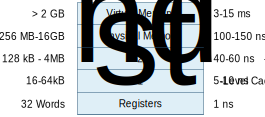
\includegraphics[width=.8\linewidth]{memory_hierarchy}
	\end{center}
\end{frame}

\begin{frame}{Locality and Memory Hierarchy}
	\begin{itemize}
	\item Locality permits to take advantage of the memory hierarchy.
	\vfill
	\item By placing the most common instructions and data in the fast-but-small storage, 
	\vfill
	\item While leaving the rest in the slow-but-large storage, we can lower the average memory-access time.
	\end{itemize}
\end{frame}

\begin{frame}{Optimization Policy}
	\begin{small}
	\begin{itemize}
	\item Put the most-recent-used instruction in the fastest memory (example of spatial locality).
	\item Put together in the same memory page/block the instructions that may be always executed together (example of spatial locality).
	\item Temporal and spatial locality of data be improved by changing:
		\begin{itemize}
		\item the data layout, or
		\item the order of the computations.
		\end{itemize}
	\end{itemize}
	\begin{example}
		\begin{itemize}
		\item For example, visiting a large amount of data and performing small operations on is not a good approach.
		\item Preferably, we should push down smaller data set into a faster memory level, and perform the computations on them.
		\end{itemize}
	\end{example}
	\end{small}
\end{frame}

\subsection{Reduction of the fragmentation}

\tableofcontentslide[sections={1-5},sectionstyle={show/shaded},subsectionstyle={show/shaded/hide},subsubsectionstyle={hide/hide/hide/hide}]

\begin{frame}{Holes in the Heap}
	\begin{itemize}
	\item At the beginning of the program, the heap is one contiguous unit of free space.
	\vfill
	\item As the program allocates and deallocates memory, this space is broken up into free and used chunks.
	\vfill
	\item The free chunks need not reside in a contiguous area of the heap.
	\vfill
	\item \emph{The free chunks are named holes.}
	\vfill
	\item Alternating chunks and holes is named the \emph{fragmentation} of the heap.
	\end{itemize}
\end{frame}

\begin{frame}{Object Placement for Minimizing the Defragmentation}
	\begin{itemize}
	\item We reduce fragmentation by controlling how the memory manager places new objects in the heap.
	\vfill
	\item Several approaches/strategies may be used:
		\vfill
		\begin{enumerate}
		\item[Best-Fit Object Placement] Allocate the requested memory in the smallest available hole that is large enough. Not good for spatial locality.
		\vfill
		\item[First-Fit Object Placement] Allocate the requested memory in the first hole, which is able to contains the requested chunk. Less efficient than the previous one.
		\vfill
		\item[Next-Fit Object Placement] When no hole of the exact size was found, allocate the in the lastly split hole. Good for spatial locality and efficient.
		\end{enumerate}
	\end{itemize}
\end{frame}

\begin{frame}{Bins in the Best-Fit Implementation}
	\begin{itemize}
	\item To improve the implementation of the best-fit approach, we introduces the \emph{bins}.
	\item \emph{Free space chunks are grouped into bins}, according to their sizes.
	\item Many bins for the smaller sizes, because there are usually many more small objects.
	\end{itemize}
	\begin{block}{\small Lea Memory Manager (GNU C compiler)}\small 
		\begin{itemize}
		\item Bins of every multiple of 8 bytes until 512 bytes.
		\item Larger-sized bins are logarithmically spaced.
		\item Within the bins the chunks are ordered by their sizes.
		\item Wilderness chunk: the largest bin because its size may be extended after requesting more memory to OS.
		\end{itemize}
	\end{block}
\end{frame}

\begin{frame}{Allocation of a Chunk}
	Let a requested chunk \code{c} to be allocated.
	\begin{enumerate}
	\item If there is a bin for chunks of the size of \code{c}, we take any free space chunk from that bin.
	\vfill
	\item\label{allocation_chunk_b} If there is no bin for chunks of the size of \code{c}, we take the smallest bin that may include the requested size. \\
		Within that bin, we can use either a first-fit or a best-fit strategy. \\
		The remainder space of the selected chunk will generally be placed in a bin with smaller size.
	\vfill
	\item If there is no more free chunk in a bin, we repeat the point \ref{allocation_chunk_b} on a bin for a larger size; or we reach the wilderness chunk, which surely provide enough space.
	\end{enumerate}
\end{frame}

\begin{frame}{Managing and Coalescing Free Space}
	\begin{itemize}
	\item When an object is deallocated, the memory manager make its chunk free.
	\item In some circumstances, it may also be possible to combine (coalesce) that freed chunk with adjacent chunks.
	\vfill
	\item Two majors data structures are basically used for supporting coalescing of adjacent free blocks:
		\begin{enumerate}
		\item \emph{Boundary Tags},
		\item \emph{Doubly Linked Free List}, Embedded Free List.
		\end{enumerate}
	\end{itemize}
\end{frame}

\sidecite{Knuth.1968}
\begin{frame}{Boundary Tags}
	\sidenote{The order of the boundary tags depends on the run-time environment}
	\begin{itemize}
	\item At both the low and high ends of a chunk, whether free or allocated, we keep vital information.
	\vfill
	\item \Emph{At both ends}, we put:
		\begin{enumerate}
		\item a bit that indicates if the chunk is free or allocated.
		\item a count of the total number of bytes in the chunk.
		\end{enumerate}
	\end{itemize}
	\vfill
	\begin{center}
		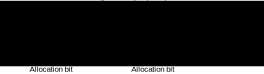
\includegraphics[width=.8\linewidth]{boundary_tags}
	\end{center}
\end{frame}

\begin{frame}{Doubly Linked Free List}
	\sidenote{The order of the boundary tags depends on the run-time environment}
	\begin{itemize}
	\item The free chunks (but not the allocated ones) are linked in a doubly linked list.
	\vfill
	\item In addition to the boundary tags, a pointer to the next and to the following free space chunks are added at the both ends of the chunk.
	\vfill
	\item Does not need to allocate more space for these pointers: the pointers takes the unused bytes of the free chunks.
	\item For the smaller chunks, they are expanded to allow to contain the pointers.
	\end{itemize}
	\vfill
	\begin{center}
		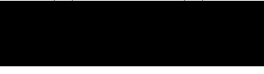
\includegraphics[width=.8\linewidth]{doubly_linked_list}
	\end{center}
\end{frame}

\subsection{Manual Deallocation}

\tableofcontentslide[sections={1-5},sectionstyle={show/shaded},subsectionstyle={show/shaded/hide},subsubsectionstyle={hide/hide/hide/hide}]

\begin{frame}{Manual Deallocation}
	\begin{itemize}
	\item This subsection is devoted to the manual deallocation requests, such as in C and C++ languages.
	\vfill
	\item Ideally, any storage that will no longer be accessed should be deleted.
	\vfill
	\item Conversely, any storage that may be referenced must not be deleted.
	\vfill
	\item It is hard to enforce these properties.
	\end{itemize}
\end{frame}

\begin{frame}{Main Problems with Manual Deallocations}
	Two common errors may occurs in manual memory management:
	\begin{enumerate}
	\vfill
	\item[Memory Leak] failing ever to delete data that cannot be referenced.
	\vfill
	\item[Dangling-pointer reference] referencing deleted data.
	\end{enumerate}
\end{frame}

\begin{frame}{Problem of Memory Leak}
	\begin{small}
	\begin{block}{\small Observation}
		\begin{itemize}
		\item It is hard for a developer to tell if a program will never refer to some storage in the future.
		\item The common mistake is not deleting storage that will never be referenced.
		\end{itemize}
	\end{block}
	\begin{alertblock}{\small Problem}
		May slow down the execution of the program due to increased memory usage.
	\end{alertblock}
	\begin{block}{\small Remarks}
		\begin{itemize}
		\item Correctness of the program is not changed.
		\item Many programs may tolerate leaks but not the long-time and the critical ones (operating systems, server code\dots)
		\end{itemize}
	\end{block}
	\end{small}
\end{frame}

\begin{frame}{Solving the Memory Leak Problem}
	\begin{enumerate}
	\item \emph{Automatic garbage collection gets rid of memory leaks by deallocating all the garbage.}\\
		Even with a garbage collector, programs may still use more memory than necessary.
	\vfill
	\item \emph{A programmer may know that an object will never be referenced.} \\
		He must deliberately remove the references to objects that will never be referenced, so the objects can be deallocated automatically.
	\end{enumerate}
\end{frame}

\begin{frame}{Problem of Dangling-Pointer Reference}
	\begin{small}
	\begin{block}{\small Observation}
		\begin{itemize}
		\item Deletion of a storage, and then referencing the deleted storage.
		\item These pointers are named ``dangling pointers.''
		\end{itemize}
	\end{block}
	\begin{alertblock}{\small Problem}
		\begin{itemize}
		\item When the storage has been reallocated, it produces random effects on the program.
		\item Writing through a dangling pointer changes an other variable than the one expecting by the dangling pointer.
		\end{itemize}
	\end{alertblock}
	\begin{block}{\small Remarks}
		Read, write or deallocate a pointer is named ``dereferencing the pointer.''
	\end{block}
	\end{small}
\end{frame}

\begin{frame}{Solving the Dangling-Pointer-Reference Problem}
	\alertbox{Unfortunately, there is no turnkey solution.}
	\begin{enumerate}
	\item \emph{The programmer must be aware and may pay attention to his uses of the pointers.}
	\vfill
	\item \emph{The dangling-pointer-dereference error does not occurs in run-time environments that has an \Emph{automatic garbage collector}.}
	\end{enumerate}
\end{frame}

\begin{frame}{Illegal Address Error}
	\begin{definition}
		This error occurs when the address to dereference is null or outside the bounds of any allocated memory (including the bounds of the memory space of the process).
	\end{definition}
	\vfill
	\begin{itemize}
	\item The illegal address error is related to the dangling-pointer-dereference error.
	\item This error is at the origin of many security violations from hackers.
	\item One solution is that the compiler inserts checks with every access, to make sure it is within the bounds.
	\item The compiler optimizer may remove several of these checks when they are detected as not necessary.
	\end{itemize}
\end{frame}

\begin{frame}[allowframebreaks]{Programming Conventions and Tools}
	\begin{block}{Object Ownership}
	\begin{itemize}
	\item Associate an owner with each object at all times.
	\item The owner is usually a function.
	\item The owner is responsible for either deleting the object or for passing the object to another owner.
	\item Non-owning points may reference the object, but the object must never be deallocated through them.
	\item This convention eliminates memory leaks, and the deletion of the same object twice.
	\item This convention does not solve the dangling-point-reference problem.
	\end{itemize}
	\end{block}
	%
	\framebreak
	%
	\begin{block}{Reference Counting}
	\begin{itemize}
	\item Associate a count with each dynamically allocated object.
	\item Whenever the reference to the object is created, the counter is incremented.
	\item Whenever the reference to the object is deleted, the counter is decremented.
	\item The storage for the object is released when the counter is zero.
	\item Expensive operation.
	\item Do not work with inaccessible circular data structures.
	\end{itemize}
	\end{block}
	%
	\framebreak
	%
	\begin{block}{Region-Based Allocation}
	\begin{itemize}
	\item When objects are created to be used only within some step of a computation, we can allocate all such objects in the same region.
	\item We then delete the entire region once that computation step completes.
	\item Limited applicability.
	\item Very efficient.
	\end{itemize}
	\end{block}
\end{frame}

\section{Garbage collection}

\tableofcontentslide[sections={2-6},sectionstyle={show/shaded},subsectionstyle={show/show/hide},subsubsectionstyle={hide/hide/hide/hide}]

\subsection{Introduction}

\sidecite{Wilson.1994}
\begin{frame}{Introduction to Garbage Collection}
	\begin{itemize}
	\item Data that cannot be referenced as named garbage.
	\item \Emph{Many high-level programming languages remove the burden of manual memory management from the programmer by offering automatic garbage collection.}
	\item The garbage collection (GC) is the process to deallocate no-more referenced storages from the heap.
	\vfill
	\item The first garbage collection dates from the initial implementation of LISP in 1958.
	\item Other languages provide natively a GC: Java, Perl, ML, Modula-3, Prolog, Smalltalk, C\#, Ruby, Python\dots
	\end{itemize}
\end{frame}

\begin{frame}{Hypothesis for Garbage Collection}
	\begin{itemize}
	\item The garbage collector must know the type of the objects at run-time. This type permits to determine:
		\begin{enumerate}
		\item the size of the object in bytes.
		\item its components that are references to other objects.
		\end{enumerate}
	\vfill
	\item The references to the objects are always to the address of the beginning of these objects.
	\item All the references to the same object have the same value and may be identified easily.
	\end{itemize}
\end{frame}

\begin{frame}{Mutator and Garbage Collection}
	\begin{definition}[Mutator]
		The mutator, the user program, modifies the collection of objects in the heap
	\end{definition}
	\vfill
	\begin{itemize}
	\item The mutator creates objects by acquiring space from the memory manager.
	\item The mutator may introduce and drop references to existing objects.
	\item Objects become garbage when the mutator program cannot ``reach'' them.
	\item The GC finds the unreachable objects and reclaims their space by handling them to the memory manager.
	\end{itemize}
\end{frame}

\subsection{Properties of a garbage collector}

\tableofcontentslide[sections={2-6},sectionstyle={show/shaded},subsectionstyle={show/shaded/hide},subsubsectionstyle={hide/hide/hide/hide}]

\begin{frame}{Type Safety}
	\begin{itemize}
	\item For a GC to work, \emph{the language must be type safe}. \\[.5em]
		The type of the data may be determined at compile or run-time.
	\vfill
	\item GC must be able to tell whether any given data element or component of a data element is, could be used as, a pointer to a chunk.
	\vfill
	\item Two family of type-safe languages:
		\begin{enumerate}
		\item[Statically typed languages] the types are determined at compile time (ML\dots)
		\item[Dynamically typed languages] the types are determined at run-time (Java\dots)
		\end{enumerate}
	\end{itemize}
\end{frame}

\begin{frame}{Unsafe Language}
	\begin{itemize}
	\item \Emph{Unsafe languages (C, C++\dots) are bad candidate for GC.}
	\vfill
	\item In unsafe languages, memory addresses can be manipulated arbitrarily (pointer arithmetic\dots)
	\vfill
	\item Thus programs can refer to any location in memory at any time.
	\vfill
	\item Consequently, no memory location can be considered to be inaccessible, and no storage can ever be reclaimed safely.
	\end{itemize}
\end{frame}

\begin{frame}{Performance Metrics}
	\begin{footnotesize}
	\begin{description}
	\item[Overall Execution Time] It is important that GC is not significantly increase the total run time of an application.
	\vfill
	\item[Space Usage] The GC must avoid fragmentation and make the best use of the available memory.
	\vfill
	\item[Pause Time] Simple GC causes the mutator to pause suddenly for an extremely long time. \\
		The maximum pause time must be minimized.
	\vfill
	\item[Program Locality] \begin{itemize}
		\item The speed of the GC cannot be evaluated solely by its running time.
		\item The GC controls the placement of data and thus influences the data locality of the mutator program.
		\item GC can improve the mutator's temporal locality by freeing the space and reusing it.
		\item It can improve the mutator's spatial locality by relocating data used together in the same cache or pages.
		\end{itemize}
	\end{description}
	\end{footnotesize}
\end{frame}

\subsection{Reachability of data}

\tableofcontentslide[sections={2-6},sectionstyle={show/shaded},subsectionstyle={show/shaded/hide},subsubsectionstyle={hide/hide/hide/hide}]

\begin{frame}{Root Set}
	\begin{definition}
		It refer to all the data that can be accessed directly by a program, without having to dereference any pointer.
	\end{definition}
	\vfill
	\begin{example}
		In Java, the root set is composed of all the static fields and all the variables in the stack.
	\end{example}
	\vfill
	\begin{description}
	\item A program can \emph{reach} any member of its root set at any time.
	\item Recursively, any object with a reference that is stored in the field members or array elements of any reachable object is itself reachable.
	\item[Note] when an object becomes unreachable, it will never be reachable again.
	\end{description}
\end{frame}

\begin{frame}[allowframebreaks]{Basic Operations to Change the Root Set}
	\begin{block}{Object allocation}
		\begin{itemize}
		\item Performed by the memory manager.
		\item The Memory manager returns a reference to each newly allocated chunk of memory.
		\item This operation adds members to the set of reachable objects.
		\end{itemize}
	\end{block}
	\begin{block}{Parameter passing and return values}
		\begin{itemize}
		\item References to objects are passed from the actual input parameter to the corresponding formal parameters; and from the returned result back to the caller.
		\item Objects pointed to by these references remain reachable.
		\end{itemize}
	\end{block}
	\begin{block}{Reference assignments}
		\begin{itemize}
		\item Assignments of the \code{x = y} (\code{x} and \code{y} are references) have two effects:
			\begin{enumerate}
			\item \code{x} is a now a reference to the object referred by \code{y}. The object referenced by \code{x} and \code{y} is reachable while \code{x} or \code{y} is reachable.
			\item The original reference of \code{x} is lost. If this lost reference is the last on the object, the object becomes unreachable.
			\end{enumerate}
		\item When an object becomes unreachable, all the reachable objects inside becomes also unreachable.
		\end{itemize}
	\end{block}
	\begin{block}{Procedure returns}
		\begin{itemize}
		\item As a procedure exists, the frame holding its local variables is popped off the stack.
		\item If the frame holds the only reachable reference to any object, that object becomes unreachable.
		\item If the now unreachable objects holds the only references to other objects, they too become unreachable, and so on.
		\end{itemize}
	\end{block}
\end{frame}

\begin{frame}[allowframebreaks]{Finding Unreachable Objects}
	\begin{enumerate}
	\item \emph{Transitions from reachability to unreachability are catched}, or \emph{the reachable objects are periodically located; assuming that all the other objects are not reachable}. \\[1em]
		Reference counting is an approximation of the first approach:
		\begin{itemize}
		\item A count of the reference to an object is maintained.
		\item When the count goes to zero, the object becomes unreachable (discussed in the next section).
		\end{itemize}
	%
	\framebreak
	%
	\item \emph{The reachability is computed by tracing all the references transitively}. \\[1em]
		\begin{itemize}
		\item A trace-based garbage collector starts by labeling, marking, all objects in the root set as ``reachable.''
		\item It examines iteratively all the references in reachable objects to find more reachable objects.
		\item It labels the discovered objects as ``reachable.''
		\item Once the reachable set is computed, it may find the unreachable objects.
		\item All the unreachable objects could be deallocated at the same time.
		\end{itemize}
	\end{enumerate}
\end{frame}

\subsection{Reference-counting garbage collector}

\tableofcontentslide[sections={2-6},sectionstyle={show/shaded},subsectionstyle={show/shaded/hide},subsubsectionstyle={show/show/hide/hide}]

\sidenote{Collins.1960}
\begin{frame}{Reference-Counting Garbage Collector}
	\begin{itemize}
	\item This section is devoted to a simple and imperfect garbage collector based on reference counting.
	\vspace{2em}
	\item With a reference-counting garbage collector, every object must have a field for the reference count; and maintains as described in the following slides.
	\end{itemize}
\end{frame}

\begin{frame}[allowframebreaks]{Actions of Reference-Counting GC}
	\begin{description}
	\item[Object allocation] The reference count of the new object is set to 1.
	\vspace{1em}
	\item[Parameter Passing] The reference count of each object passed into a procedure is incremented.
	\vspace{1em}
	\item[Reference Assignments] For statement \code{u=v} (\code{u} and \code{v} are references), the reference count of the object referred to by \code{v} goes up by one, and the count for the old object referred to by \code{u} goes down by one.
	%
	\framebreak
	%
	\item[Procedure Returns] As a procedure exsits, objects referred to by the local variables in its activation record have their counts decremented. If several local variables hold references to the same object, that object's count must be incremented once for each such reference.
	\vspace{1em}
	\item[Transitive Loss of Reachability] Whenever the reference count of an object becomes zero, we mist also decrement the count of each object pointed to by a reference within the object.
	\end{description}
\end{frame}

\begin{frame}<-11>[t,fragile]{Example of Reference-Counting Garbage Collector}
	\begin{lstlisting}[linewidth={.35\linewidth},language=java,basicstyle=\tiny,backgroundcolor={}]
		class Obj {
		   public Obj a = null;
		   public Obj b = null;
		}
		class Main {
		   public static void main(String[] args) {
		      Obj o1 = new Obj();
		      {
		         Obj o2 = new Obj();
		         Obj o3 = new Obj();
		         o1.b = o2;
		         o2.a = o1;
		         o2.b = o3;
		         o3.b = o1;
		      }
		   }
		}
	\end{lstlisting}
	\putat(130,-200){\includeanimatedfigure[width=.4\paperwidth]{reference_counting_exemple}}
	\only<2>{\putat(-30,-79){\pgfuseimage{rightarrow}}}
	\only<3>{\putat(-30,-94){\pgfuseimage{rightarrow}}}
	\only<4>{\putat(-30,-100){\pgfuseimage{rightarrow}}}
	\only<5>{\putat(-30,-107){\pgfuseimage{rightarrow}}}
	\only<6>{\putat(-30,-115){\pgfuseimage{rightarrow}}}
	\only<7>{\putat(-30,-121){\pgfuseimage{rightarrow}}}
	\only<8>{\putat(-30,-129){\pgfuseimage{rightarrow}}}
	\only<9>{\putat(-30,-135){\pgfuseimage{rightarrow}}}
	\only<10>{\putat(-30,-142){\pgfuseimage{rightarrow}}}
	\only<11>{\putat(130,-18){\parbox[t]{.5\paperwidth}{\normalcolor\mdseries\small\nohyphens{
		This set of objects should be garbage collected. But their counters are greater than 0. Such a situation is tantamount to a \alert{memory leak}, since this set of objects will never be deallocated.}}}}
\end{frame}

\begin{frame}<12->[t,fragile]{Solving Memory Leak with Reference-Counting Garbage Collector}
	\begin{lstlisting}[linewidth={.35\linewidth},language=java,basicstyle=\tiny,backgroundcolor={}]
		class Obj {
		   public Obj a = null;
		   public Obj b = null;
		}
		class Main {
		   public static void main(String[] args) {
		      Obj o1 = new Obj();
		      {
		         Obj o2 = new Obj();
		         Obj o3 = new Obj();
		         o1.b = o2;
		         o2.a = o1;
		         o2.b = o3;
		         o3.b = o1;
		      }
		      o1.b = null;
		   }
		}
	\end{lstlisting}
	\putat(130,-200){\includeanimatedfigure[width=.4\paperwidth]{reference_counting_exemple}}
	\only<12-13>{\putat(-30,-143){\pgfuseimage{rightarrow}}}
	\only<14>{\putat(-30,-150){\pgfuseimage{rightarrow}}}
	\only<12>{\putat(130,-18){\parbox[t]{.5\paperwidth}{\normalcolor\mdseries\small\nohyphens{
		A line is added to reset the reference from \code{o1} to \code{o2}.}}}}
	\only<15>{\putat(130,-18){\parbox[t]{.5\paperwidth}{\normalcolor\mdseries\small\nohyphens{
		The chunk, previously refered by \code{o2}, is no more referenced. It is garbage collected.}}}}
	\only<16>{\putat(130,-18){\parbox[t]{.5\paperwidth}{\normalcolor\mdseries\small\nohyphens{
		Chunk refered by \code{o3} is garbage collected.}}}}
	\only<17>{\putat(130,-18){\parbox[t]{.5\paperwidth}{\normalcolor\mdseries\small\nohyphens{
		Chunk refered by \code{o1} is garbage collected. There is \emph{no memory leak}.}}}}
\end{frame}

\begin{frame}{Deferred Reference Counting}
	\begin{itemize}
	\item The concept of \emph{deferred reference counting} has been proposed as a mean to eliminate the overhead associated with updating the reference counts due to stack accesses.
	\vfill
	\item Reference counts do not include references from the root set of the program.
	\item An object is not considered to be garbage until the entire root set is scanned and no reference to the object is found.
	\end{itemize}
\end{frame}

\begin{frame}{Advantages of Reference Counting}
	\begin{enumerate}
	\item Garbage Collection is performed in an \emph{incremental fashion}.
		\begin{itemize}
		\item The operations are made through the mutator's operations.
		\item Removing one reference may render a large number of objects unreachable, the operation of recursively modifying reference counts can easily be deferred and performed piecemeal across time.
		\item Reference counting is particularly attractive when timing deadlines must be met.
		\end{itemize}
	\vfill
	\item Garbage are collected immediately, keeping space usage low.
	\end{enumerate}
\end{frame}

\begin{frame}{Disadvantages of Reference Counting}
	\begin{enumerate}
	\item Reference counting cannot collect unreachable, cyclic data structures.
		\begin{itemize}
		\item Cyclic data structures are quite plausible.
		\item Data structures often point back to their parent nodes, or point to each other as cross references.
		\end{itemize}
	\vfill
	\item Overhead of reference counting is high:
		\begin{itemize}
		\item Additional operations were introduced with each reference assignment.
		\item Additional operations were introduced with each procedure call and exit.
		\item The overhead is proportional to the amount of computation in the program, and not just to the number of objects in the system.
		\end{itemize}
	\end{enumerate}
\end{frame}

\subsection{Trace-based garbage collector}

\subsubsection{Introduction}

\tableofcontentslide[sections={4-6},sectionstyle={show/shaded},subsectionstyle={show/shaded/hide},subsubsectionstyle={show/show/hide/hide}]

\sidecite{McCarthy.1960}
\begin{frame}{Trace-Based Garbage Collector}
	\begin{itemize}
	\item Instead of collecting garbage as it is created, trace-based collectors run periodically to find unreachable objects.
	\vfill
	\item Typically, we run the trace-based collector whenever the free space is exhausted or its amount drops below some threshold.
	\vfill
	\item All trace-based algorithms:
		\begin{enumerate}
		\item compute the set of reachable objects, and
		\item Take the complement of this list.
		\end{enumerate}
	\end{itemize}
\end{frame}

\begin{frame}{States of the Chunks}
	\begin{definition}[Free]
		\begin{itemize}
		\item A chunk is in the \emph{Free} state if it is ready to be allocated.
		\item A Free chunk must not hold a reachable object.
		\end{itemize}
	\end{definition}
	\begin{definition}[Allocated]
		\begin{itemize}
		\item A chunk is in the \emph{Allocated} state if it was used to store data.
		\item An allocated chunk must be in one of the three substates:
			\begin{enumerate}
			\item Unreached
			\item Unscanned
			\item Scanned
			\end{enumerate}
		\end{itemize}
	\end{definition}
	\begin{center}
		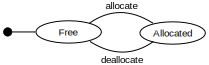
\includegraphics[width=.5\linewidth]{chunk_states}
	\end{center}
\end{frame}

\begin{frame}[t]{States of an Allocated Chunk}
	\begin{footnotesize}
	\only<1>{\begin{definition}[Unreached]
		\begin{itemize}
		\item Chunks are presumed unreachable, unless proven reachable by tracing.
		\item A chunk is in the \emph{Unreached} state at any point during garbage collection if its reachability has not yet been established.
		\item After a round of garbage collection, the state of a reachable object is reset to Unreachable to get ready for the next round (see the next states).
		\end{itemize}
	\end{definition}}
	\only<2>{\begin{definition}[Unscanned]
		\begin{itemize}
		\item A chunk is in the \emph{Unscanned} state if it is known as be reachable, but its pointers have not yet been scanned.
		\item The transition to Unscanned from Unreached occurs when we discover that a chunk is reachable.
		\end{itemize}
	\end{definition}}
	\only<3>{\begin{definition}[Scanned]
		\begin{itemize}
		\item Every Unscanned object will eventually be scanned and transition to the \emph{Scanned} state.
		\item To scan an object, we examine each of the pointers within it and follow those pointers to the objects to which they refer.
		\item A scanned object can only contain references to other scanned ot unscanned objects, never to unreached objects. Consequently, the accessible chunks are moved to the Unscanned state if they are unreachable.
		\end{itemize}
	\end{definition}}
	\end{footnotesize}
	\only<4>{\begin{itemize}
		\item At the end of its algorithm, the GC is deallocating the unreached chunks.
		\item It is setting the states of the reached chunks to ``Unreached'' for the next GC execution.
		\end{itemize}}
	\putat(50,-210){\includeanimatedfigure[width=.7\linewidth]{allocated_chunk_states}}
\end{frame}

\subsubsection{Basic mark-and-sweep collector}

\tableofcontentslide[sections={4-6},sectionstyle={show/shaded},subsectionstyle={show/shaded/hide},subsubsectionstyle={show/shaded/hide/hide}]

\sidecite{McCarthy.1960}
\begin{frame}{Mark-and-Sweep Collector}
	\begin{itemize}
	\item Mark-and-sweep collectors are \Emph{``stop-the-world''} algorithms.
	\item They find all the unreachable objects, and put them on the list of free space.
	\vfill
	\item The algorithm visits and ``marks'' all the reachable objects in the first tracing step.
	\item Then it ``sweeps'' the entire heap to free up unreachable objects.
	\end{itemize}
\end{frame}

\begin{frame}[t,allowframebreaks]{Algorithm of the Mark-and-Sweep Collector}
	\begin{footnotesize}
	\begin{myalgorithm}
	\SetKwBlock{myBeginBlock}{begin}{}
	\SetKwFunction{copyof}{copy-of}%
	\SetKwFunction{referencesin}{references\_in}%
	\Input{A root set of objects, a heap, and a free list (named \code{Free}), with all the unallocated chunks of the heap.}
	\Output{A modified \code{Free} list after all the garbage has been removed.}
	\myBeginBlock{
		\tcc{MARKING PHASE}
		Unscanned \affect \copyof{root}\;
		\ForEach{o $\in$ Unscanned}{
			reached\_bit[o] \affect false\;
		}
		\While{$\exists$ o $\in$ Unscanned}{
			Unscanned \affect Unscanned $\setminus \{ o \}$\;
			\ForEach{r $\in$ \referencesin{o}}{
				\If{$neg$ reached\_bit[r]}{
					reached\_bit[r] \affect true\;
					Unscanned \affect Unscanned $\cup \{ r \}$\;
				}
			}
		}
	}
	\end{myalgorithm}
	\end{footnotesize}
	%
	\begin{footnotesize}
	\begin{myalgorithm}
	\SetKwBlock{myEndBlock}{}{end}
	\myEndBlock{
		\tcc{SWEEPING PHASE}
		Free \affect $\emptyset$\;
		\ForEach{c $\in$ chunks}{
			\uIf{$neg$ reached\_bit[c]}{
				Free \affect Free $\cup \{ c \}$\;
			}
			\Else{
				reached\_bit[c] \affect false\;
			}
		}
	}
	\end{myalgorithm}
	\end{footnotesize}
\end{frame}

\begin{frame}{Optimizing Mark-and-Sweep Collector}
	\begin{alertblock}{Problem}
		\begin{itemize}
		\item The final step in the mark-and-sweep algorithm is expensive.
		\item Not easy way to find the unreachable objects without examining the entire heap.
		\end{itemize}
	\end{alertblock}
	\vfill
	\begin{block}{Improved Algorithm}
		\begin{itemize}
		\item \Emph{Baker's Mark-and-sweep Algorithm.}
		\item It keeps a list of all allocated objects and compute a difference between the allocated objects and the reached objects.
		\end{itemize}
	\end{block}
\end{frame}

\sidecite{Baker.1992}
\begin{frame}[t,allowframebreaks]{Baker's Algorithm of the Mark-and-Sweep Collector}
	\begin{scriptsize}
	\begin{myalgorithm}
	\SetKwBlock{myBeginBlock}{begin}{}
	\SetKwFunction{referencesin}{references\_in}%
	\Input{A root set of objects, a heap, a free list (named \code{Free}), a listo f allocated objects \code{Unreached}.}
	\Output{A modified \code{Free} and \code{Unreached} lists.}
	\myBeginBlock{
		\tcc{MARKING PHASE}
		Unscanned \affect $\emptyset$\;
		Scanned \affect $\emptyset$\;
		\ForEach{o $\in$ root $\cap$ Unreached}{
			Unreached \affect Unreached $\setminus \{ o \}$; Unscanned \affect Unscanned $\cup \{ o \}$\;
		}
		\While{$\exists$ o $\in$ Unscanned}{
			Unscanned \affect Unscanned $\setminus \{ o \}$\;
			Scanned \affect Scanned $\cup \{ o \}$\;
			\ForEach{r $\in$ \referencesin{o}}{
				\If{r $\in$ Unreached}{
					Unreached \affect Unreached $\setminus \{ r \}$\;
					Unscanned \affect Unscanned $\cup \{ r \}$\;
				}
			}
		}
	}
	\end{myalgorithm}
	\end{scriptsize}
	\begin{scriptsize}
	\begin{myalgorithm}
	\SetKwBlock{myEndBlock}{}{end}
	\myEndBlock{
		\tcc{SWEEPING PHASE}
		Free \affect Free $\cup$ Unreached\;
		Unreached \affect Scanned\;
	}
	\end{myalgorithm}
	\end{scriptsize}
\end{frame}

\subsubsection{Mark-and-compact garbage collector}

\tableofcontentslide[sections={4-6},sectionstyle={show/shaded},subsectionstyle={show/shaded/hide},subsubsectionstyle={show/shaded/hide/hide}]

\begin{frame}{Relocating Collectors}
	\begin{itemize}
	\item Relocating collectors move reachable objects around in the heap to eliminate memory fragmentation.
	\item After identifying all the holes, instead of freeing them, one alternative is to relocate the allocated objects in one end of the heap.
	\item The rest of the memory becomes a single free chunk.
	\vfill
	\item Two major approaches for building a relocating collector are:
		\begin{enumerate}
		\item A \emph{mark-and-compact collector}
		\item A \emph{copying collector}
		\end{enumerate}
	\end{itemize}
\end{frame}

\begin{frame}{Mark-and-Compact Collectors}
	The mark-and-compact collector follows:
	\vfill
	\begin{enumerate}
	\item[Marking Phase] similar to the mark-and-sweep algorithms
	\vfill
	\item[Object Relocation] \begin{itemize}
		\item The allocated regions of the heap are scanned.
		\item The address of each reachable object is computed from the low end of the heap.
		\item The addresses are stored in a structure named \code{NewLocation}.
		\end{itemize}
	\vfill
	\item[Object Copy] \begin{itemize}
		\item The objects are copied to their new locations,
		\item The references in the objects to point to are updated.
		\end{itemize}
	\end{enumerate}
\end{frame}

\begin{frame}[t,allowframebreaks]{Algorithm of the Mark-and-Compact Collector}
	\begin{footnotesize}
	\begin{myalgorithm}
	\SetKwFunction{copyof}{copy\_of}%
	\SetKwFunction{referencesin}{references\_in}%
	\SetKwBlock{myBeginBlock}{begin}{}
	\Input{A root set of objects, a heap, a pointer marking the start of the free space (named \code{Free}).}
	\Output{The new value of pointer \code{Free}}
	\myBeginBlock{
		\tcc{MARKING PHASE}
		Unscanned \affect \copyof{root}\;
		\ForEach{o $\in$ Unscanned}{
			reached\_bit[o] \affect false\;
		}
		\While{$\exists$ o $\in$ Unscanned}{
			Unscanned \affect Unscanned $\setminus \{ o \}$\;
			\ForEach{r $\in$ \referencesin{o}}{
				\If{$neg$ reached\_bit[r]}{
					reached\_bit[r] \affect true\;
					Unscanned \affect Unscanned $\cup \{ r \}$\;
				}
			}
		}
	}
	\end{myalgorithm}
	\end{footnotesize}
	\begin{footnotesize}
	\begin{myalgorithm}
	\SetKwFunction{sizeof}{size\_of}%
	\SetKwBlock{myBlock}{}{}
	\myBlock{
		\tcc{COMPUTE THE NEW LOCATIONS}
		NewLocation \affect $[]$\;
		Free \affect first address in the heap;
		\ForEach{c $\in$ chunks[0..]}{
			\If{reached\_bit[c]}{
				NewLocation[c] \affect Free\;
				Free \affect Free \sizeof{c}\;
			}
		}
	}
	\end{myalgorithm}
	\end{footnotesize}
	\begin{footnotesize}
	\begin{myalgorithm}
	\SetKwFunction{referencesin}{references\_in}%
	\SetKwBlock{myEndBlock}{}{end}
	\myEndBlock{
		\tcc{RETARGET THE REFERENCES AND MOVE REACHED OBJECTS}
		\ForEach{c $\in$ chunks[0..]}{
			\If{reached\_bit[c]}{
				\ForEach{r $\in$ \referencesin{c}}{
					c.r \affect NewLocation[c.r]\;
				}
				Copy c to NewLocation[c]\;
			}
		}
		\ForEach{r $\in$ \referencesin{root}}{
			r \affect NewLocation[r]
		}
	}
	\end{myalgorithm}
	\end{footnotesize}
\end{frame}

\subsubsection{Copying collector}

\tableofcontentslide[sections={4-6},sectionstyle={show/shaded},subsectionstyle={show/shaded/hide},subsubsectionstyle={show/shaded/hide/hide}]

\sidecite{Fenichel.1969, Cheney.1970}
\begin{frame}{Copying Collectors}
	\begin{itemize}
	\item A copying collector reserves space to which hthe objects can move.
	\item The memory space is partitioned into two semispaces $A$ and $B$.
	\item The mutator allocates in $A$ until it fill up.
	\item Then the mutator is stopped and the GC copies the reachable objects to $B$.
	\item When GC finished, the roles of $A$ and $B$ are reversed.
	\vfill
	\item The algorithm is due to C.J. Cheney.
	\end{itemize}
\end{frame}

\subsubsection{Brief Comparison}

\tableofcontentslide[sections={4-6},sectionstyle={show/shaded},subsectionstyle={show/shaded/hide},subsubsectionstyle={show/shaded/hide/hide}]

\begin{frame}{Comparing the Costs}
	\begin{description}
	\item[Basic Mark-and-sweep] Proportional to the number of chunks in heap.
	\vfill
	\item[Baker's Mark-and-sweep] Proportional to the number of reached objects.
	\vfill
	\item[Basic Mark-and-compact] Proportional to the number of chunks in the heap plus the total size of the reached objects.
	\vfill
	\item[Cheney's Copying Collector] Proportional to the total of the reached objects.
	\end{description}
\end{frame}

\subsection{Short-pause garbage collector}

\tableofcontentslide[sections={4-6},sectionstyle={show/shaded},subsectionstyle={show/shaded/hide},subsubsectionstyle={show/show/hide/hide}]

\subsubsection{Introduction}

\begin{frame}{Be Better Than Trace-based Collectors}
	\begin{alertblock}{Problem of the trace-based collectors}
		\begin{itemize}
		\item Trace-based collectors do \emph{stop-the-world} GC.
		\item It may introduce long pauses into execution of user programs.
		\end{itemize}
	\end{alertblock}
	\vfill
	\begin{block}{First Solution: Incremental Collection}
		Divide the work in time, by interleaving GC with the mutation.
	\end{block}
	\vfill
	\begin{block}{Second Solution: Partial Collection}
		Divide the work in space, by collecting a subset of the garbage at a time.
	\end{block}
\end{frame}

\subsubsection{Incremental garbage collector}

\tableofcontentslide[sections={4-6},sectionstyle={show/shaded},subsectionstyle={show/shaded/hide},subsubsectionstyle={show/shaded/hide/hide}]

\begin{frame}{Incremental Garbage Collection}
	\begin{itemize}
	\item Incremental collectors are conservative:
		\begin{itemize}
		\item While GC must not collect objects that are not garbage,
		\item It does not have to collect all the garbage in each round.
		\end{itemize}
	\vfill
	\item The garbage left in memory is named \emph{floating garbage}.
	\item Incremental collectors overestimate the set of reachable objects.
	\end{itemize}
\end{frame}

\begin{frame}{Incremental Algorithm}
	\begin{enumerate}
	\item The program's root set is processed automatically, without interference with the mutator.
	\vfill
	\item After finding the initial set of unscanned objects, the mutator's actions are interleaved with the tracing step.
	\vfill
	\item During this period, any of the mutator's actions that may change reachability are recorded succinctly, in a side table.
	\vfill
	\item The side table is used by the collector to adjust the memory allocation when the mutator's actions resume their execution.
	\vfill
	\item If there is not enough memory space, the collector blocks the mutator until it finished to collect the garbage.
	\end{enumerate}
\end{frame}

\begin{frame}{Reachable Objects}
	The set of reachable objects when tracing finished is:
		\[ \left( R \cup New \right) \setminus Lost \]
	\vfill
	\begin{itemize}
	\item $R$: the set of reachable objects at the beginning of garbage collection.
	\item $New$: the set of allocated objects during garbage collection.
	\item $Lost$:  the set of objects that have become unreachable due to lost references.
	\end{itemize}
\end{frame}

\begin{frame}{Problem of the Computation of the Reachable Objects}
	\begin{itemize}
	\item \alert{It is expensive to compute an object's reachability every time.}
	\vfill
	\item Incremental collectors do not attempt to collect all the garbages at the end of the tracing.
	\item Every garbage left behind (floating garbage) should be a subset of the Lost objects.
	\end{itemize}
	\vfill
		\[ \left( \left( R \cup New \right) \setminus Lost \right) \subseteq S \subseteq \left( R \cup New \right) \]
\end{frame}

\begin{frame}{Basic Incremental Algorithm}
	\begin{itemize}
	\item First, we use a tracing algorithm to find the upper bounds of $R \cup New$. 
	\item The behavior of the mutator is modified during the tracing:
		\begin{itemize}
		\item All references that existed before GC are preserved.
		\item All objects created are considered reachable immediately and are placed in the Unscanned state.
		\end{itemize}
	\item This scheme is conservative and finds $R$ and $New$.
	\end{itemize}
	\vfill
	\alertbox{But the cost is high because the algorithm intercept all the write operations and remembers all the overwritten references.}
	\vfill
	\alertbox*{The following slides proposes a solution.}
\end{frame}

\sidecite{Dikjstra.1978}
\begin{frame}{Incremental Reachability Analysis}
	\begin{itemize}
	\item If mutator and tracing GC algorithm are interleaved, then some reachable objects may be misclassified as unreachable.
	\vfill
	\item Because the mutator may violate the following invariant of the GC algorithm: \\
		A scanned object can only contain references to other scanned or unscanned objects, never unreached objects.
	\end{itemize}
\end{frame}

\begin{frame}[t]{Examples of Violation}
	\begin{small}
	\begin{itemize}
	\item<1> The garbage collector find object $A$ reachable and scans the pointers within $A$, thereby putting $A$ in the Scanned state.
	\item<2> The mutator stores a reference to an Unreached (but reachable) object $B$ into the Scanned object $A$. It does so by copying a reference to $B$ from an object $C$ that is currently in the Unreached or Unscanned state.
	\item<3> The mutator loses the reference to $B$ in object $C$. It may have overwritten $C$'s reference to $B$ before the reference is scanned, or $C$ may have become unreachable and never have reached the Unscanned state to have its reference scanned.
	\end{itemize}
	\end{small}
	\vfill
	\begin{center}
		\includeanimatedfigure[width=.8\linewidth]{violation}
	\end{center}
\end{frame}

\begin{frame}[allowframebreaks]{Avoiding the Violations}
	\begin{small}
	\begin{description}
	\item[Write Barriers] \begin{itemize}
		\item Intercepts writes of references into a Scanned object $A$.
		\item When the reference is to an Unreached object $B$, then classify the object $B$ as reachable and place it in an Unscanned state;
		\item or put the object $A$ in an Unscanned state.
		\end{itemize}
	\item[Read Barriers] \begin{itemize}
		\item Intercept the reads of references in Unreached or Unscanned objects.
		\item When the mutator reads the reference to object A from an object in Unreached or Unscanned state, classify A as reachable and put it in the Unscanned state.
		\end{itemize}
	%
	\framebreak
	%
	\item[Transfer Barriers] \begin{itemize}
		\item Intercept the loss of the original reference in an Unreached or Unscanned object.
		\item When the mutator overwrites a reference in an Unreached or Unscanned object, save the reference being overwritten, classify it as reachable, and place the reference itself in the Unscanned state.
		\end{itemize}
	\end{description}
	\end{small}
\end{frame}

\begin{frame}{Comparison of the Mutator Barriers}
	\begin{itemize}
	\item Write barriers are the most efficient of the barriers.
	\vfill
	\item Read barriers are more expensive because typically there are many more reads than there are writes.
	\vfill
	\item Transfer barriers are not competitive; because many objects ``die young,'' this approach would retain many unreachable objects.
	\end{itemize}
\end{frame}

\subsubsection{Partial garbage collector}

\tableofcontentslide[sections={4-6},sectionstyle={show/shaded},subsectionstyle={show/shaded/hide},subsubsectionstyle={show/shaded/hide/hide}]

\begin{frame}{Partial Garbage Collector}
	\begin{itemize}
	\item Fact: ``Objects typically die young.''
	\item These objects becomes unreachable before the GC is invoked.
	\item Consequently, GC is cost effective with the approaches presented in the previous slides.
	\item The same ``mature'' objects were found and copied at every round of the GC.
	\vfill
	\item Two major approaches make partial GC to be more effective:
		\begin{enumerate}
		\item Generational GC
		\item Train Algorithm
		\end{enumerate}
	\end{itemize}
\end{frame}

\sidecite{Lieberman.1983}
\begin{frame}{General Principle of the Generational GC}
	\begin{itemize}
	\item The heap is divided in partitions: 0, 1, \dots, n (0 is for the younger data)
	\vfill
	\item Objects are created in partition 0.
	\vfill
	\item When the partition 0 fills up, it is GC and the reachable objects are moved in partition 1.
	\vfill
	\item The same algorithm is used between partition 1 and 2, 2 and 3\dots
	\end{itemize}
\end{frame}

\sidecite{Hudson.1992}
\begin{frame}{Car and Train Definitions}
	\begin{itemize}
	\item The train algorithm uses fixed-length partitions, called \emph{cars}.
	\end{itemize}
	\begin{definition}[Car]
		\begin{itemize}
		\item A car might be a single disk block, assuming there are no object larger than disk blocks; or
		\item the car size could be larger, but it is fixed once and for all.
		\end{itemize}
	\end{definition}
	\begin{definition}[Train]
		Cars are organized into trains. There is no limit to the number of cars in a train, and no limit to the number of trains.
	\end{definition}
\end{frame}

\begin{frame}{General Principles of the Train Algorithm}
	Two approaches to collect the garbages:
	\begin{enumerate}
	\item<1> The first car in lexicographic order is collected in one incremental garbage-collection step. \begin{itemize}
		\item This step is similar to collection of the first partition in the generational algorithm, since we maintain a ``remembered'' list of all points from outside the car.
		\item We identify objects with no references at all, as well as garbage cycles that are contained completely within this car.
		\item Reachable objects in the car are always moved to some other car, so each garbage-collected car becomes empty and can be removed from the train.
		\end{itemize}
	\item<2> Sometimes, the first train has no external reference. \begin{itemize}
		\item That is, there are no pointers from the root set to any car of the train, and the remembered sets for the cars contain only references from other cars in the train, not from other trains.
		\item In this situation, the train is a huge collection of cyclic garbage, and we delete the entire train.	
		\end{itemize}
	\end{enumerate}
\end{frame}

\begin{frame}{Generational GC vs. Train Algorithm}
	\begin{itemize}
	\item Generational GC works most frequently on the area of the heap that contains the youngest objects. \\
		It tends to collect a lot of garbage for relatively little work.
	\vfill
	\item The train algorithm does not spend a large proportion of time on young objects. \\
		It does limit the pauses due to garbage collection. \\
		An advantage to the train algorithm is that we never have to do a complete garbage collection, as we do occasionally for generational garbage collection.
	\vfill
	\item A good combination of strategies is to use generational collection  for young objects, and once an becomes sufficiently mature, to ``promote'' it to a separate heap that is managed by the train algorithm.
	\end{itemize}
\end{frame}

\section{Conclusion}

\tableofcontentslide[sectionstyle={show/shaded},subsectionstyle={hide/hide/hide},subsubsectionstyle={hide/hide/hide/hide}]

\begin{frame}[t,allowframebreaks]{Key Concepts in the Chapter}
	\begin{small}
	\begin{description}
	\item[Run-time Organization] To implement the abstractions embodied in the source language, a compiler creates and manages a run-time environment in concert with the operating system and the target machine. The run-time environment has static data areas for the object code and the static data objects created at compile time. It also has dynamic stack and heap areas for managing objects created and destroyed as the target program executes.
	\item[Control Stack]  Procedure calls and returns are usually managed by a run-time stack called the \emph{control stack}. We can use a stack because procedure calls or \emph{activations} nest in time; that is, if \code{p} calls \code{q}, then this activation of \code{q} is nested within this activation of \code{p}.
	\item[Stack Allocation] Storage for local variables can be allocated on a run-time stack for languages that allow or require local variables to become inaccessible when their procedures end. For such languages, each live activation has an \emph{activation record} (or \emph{frame}) on the control stack, with the root of the activation tree at the bottom, and the entire sequence of activation records on the stack corresponding to the path in the activation tree to the activation where control currently resides. The latter activation has its record at the top of the stack.
	\item[Access to Nonlocal Data on the Stack] For languages like C that do not allow nested procedure declarations, the location for a variable is either global or found in the activation record on top of the run-time stack. For languages with nested procedures, we can access nonlocal data on the stack through \emph{access links}, which are pointers added to each activation record. The desired nonlocal data is found by following a chain of access links to the appropriate activation record. A \emph{display} is an auxiliary array, used in conjunction with access links, that provides an efficient short-cut alternative to a chain of access links.
	\item[Heap Management] The \emph{heap} is the portion of the store that is used for data that can live indefinitely, or until the program deletes it explicitly. The \emph{memory manager} allocates and deallocates space within the heap. \emph{Garbage collection} finds spaces within the heap that are no longer in use and can therefore be reallocated to house other data items. For languages that require it, the garbage collector is an important subsystem of the memory manager.
	\item[Exploiting Locality] By making good use of the memory hierarchy, memory managers can influence the run time of a program. The time taken to access different parts of memory can vary from nanoseconds to milliseconds. Fortunately, most programs spend most of their time executing a relatively small fraction of the code and touching only a small fraction of the data. A program has \emph{temporal locality} if it is likely to access to same memory locations again soon; it has \emph{spatial locality} if it is likely to access nearby memory locations soon.
	\item[Reducing Fragmentation] As the program allocates and deallocates memory, the heap may get \emph{fragmented}, or broken into large numbers of small noncontiguous free spaces or holes. The best fit strategy (allocate the smallest available hole that satisfies a request) has been found empirically to work well. While best fit tends to improve space utilization, it may not be best for spatial locality. Fragmentation can be reduced by combining or \emph{coalescing} adjacent holes.
	\item[Manual Deallocation] Manual memory management has two common failings: not deleting data that can not be referenced is a \emph{memory-leak} error, and referencing deleted data is a \emph{dangling-pointer-reference} error.
	\item[Reachability] \emph{Garbage} is data that cannot be referenced or reached. There are two basic ways of finding unreachable objects: either catch the transition as a reachable object turns unreachable, or periodically locate all the reachable objects and infer that all remaining objects are unreachable.
	\item[Reference-Counting Collectors] maintain a count of the references to an object; when the count transitions to zero, the object becomes unreachable. Such collectors introduce the overhead of maintaining references and can fail to find ``cyclic'' garbage, which consists of unreachable objects that reference each other, perhaps through a chain of references.
	\item[Trace-Based Garbage Collectors] iteratively examine or trace all references to find reachable objects, starting with the \emph{root set} consisting of objects that can be accessed directly without having to dereference any pointers.
	\item[Mark-and-Sweep Collectors] visit and mark all reachable objects in a first tracing step and then sweep the heap to free up unreachable objects.
	\item[Mark-and-Compact Collectors] improve upon mark-and-sweep; they \emph{relocate} objects in the heap to eliminate memory fragmentation.
	\item[Copying Collectors] break the dependency between tracing and finding free space. They partition the memory into two \emph{semispaces}, A and B. Allocation requests are satisfied from one semispace, say A, until it fills up, at which point the garbage collector takes over, copies the reachable objects to the other space, say B, and reverses the roles of the semispaces.
	\item[Incremental Collectors] Simple trace-based collectors stop the user program while garbage is collected. \emph{Incremental collectors} interleave the actions of the garbage collector and the \emph{mutator} or user program. The mutator can interfere with incremental reachability analysis, since it can change the references within previously scanned objects. Incremental collectors therefore play it safe by overestimating the set of reachable objects; any ``floating garbage'' can be picked up in the next round of collection.
	\item[Partial Collectors] also reduce pauses; they collect a subset of the garbage at a time. The best known of partial-collection algorithms, \emph{generational garbage collection}, partitions objects according to how long they have been allocated and collects the newly created objects more often because they tend to have shorter lifetimes. An alternative algorithm, the \emph{train algorithm}, uses fixed length partitions, called cars, that are collected into \emph{trains}. Each collection step is applied to the first remaining car of the first remaining train. When a car is collected, reachable objects are moved out to the other cars, so this car is left with garbage and can be removed from the train. These two algorithms can be used together to create a partial collector that applies the generational algorithm to younger objects and the train algorithm to more mature objects.
	\end{description}
	\end{small}
\end{frame}

\begin{frame}[t,allowframebreaks]{\bibname\ of the Chapter}%
	\tiny%
	\putbib[bibliographies/chapter5]%
\end{frame}%

\end{bibunit}

